% DAI 701 SLR -- acmart skeleton (Overleaf fallback).
% Every [YOU] / TODO [YOU] is author-written content. This file holds structure only, no manuscript text.
% Section order follows the handout; each section's requirements are listed in its file under sections/.
\documentclass[manuscript,screen,review]{acmart}

% Course paper: switch off the ACM rights and reference-format boilerplate.
\setcopyright{none}
\settopmatter{printacmref=false}
\renewcommand\footnotetextcopyrightpermission[1]{}

% acmart already loads hyperref, graphicx and booktabs: do not load hyperref again.
\usepackage{booktabs}
\usepackage{xurl}
\usepackage{tikz}
\usepackage{listings}
\lstset{basicstyle=\ttfamily\scriptsize, breaklines=true, breakatwhitespace=true, columns=fullflexible}
\usetikzlibrary{positioning,arrows.meta,shapes}

% \comparisontable{<caption>}{<label>}{<column spec>}{<header cells>}{<body rows, each ending in \\>}
\newcommand{\comparisontable}[5]{%
  \begin{table}[htbp]
    \caption{#1}\label{#2}
    \small
    \begin{tabular}{#3}
      \toprule
      #4 \\
      \midrule
      #5
      \bottomrule
    \end{tabular}
  \end{table}}

\begin{document}

% TODO [YOU] title
\title{[YOU]}

% TODO [YOU] author name
\author{[YOU]}
\affiliation{%
  \institution{Ajman University}
  \city{Ajman}
  \country{United Arab Emirates}}

% TODO [YOU] abstract, 150--250 words: precise scope, the review's RQs, method, headline findings.
\begin{abstract}
[YOU]
\end{abstract}

% TODO [YOU] CCS concepts: generate the CCSXML block and \ccsdesc lines at https://dl.acm.org/ccs and paste them here.
% \ccsdesc[500]{[YOU]}

% TODO [YOU] 4--6 keywords
\keywords{[YOU]}

\maketitle

\section{Introduction}\label{sec:introduction}
% Must contain: motivation; scope and boundaries; the review's research questions; why existing surveys
% are insufficient (optionally a table comparing prior surveys: what they covered, their gaps, what this review adds);
% the contributions of this review; a roadmap of the paper.

% The following framing was written by the author on 2026-10-31.
\subsection{Motivation and Problem Statement}
Current research on LLM cybersecurity agents is difficult to evaluate because results often rely on small, puzzle-style task sets and incompletely disclosed scaffolding choices that blur what the model contributes and what the harness contributes. Public challenge material also creates a plausible contamination risk, although the reviewed evidence does not establish memorization as the cause of any reported result. Missing human and tool baselines, binary success metrics, and limited frontier-model disclosure further constrain comparison and reproducibility. Verified examples include conflicting hold-out results, unreconciled aggregate success rates, and human-mediated scores that cannot be read as autonomous end-to-end performance~\cite{R0322_Wu_2025,R0320_Huang_2025,R0384_Xiao_2025}.

\subsection{Why This Review Is Timely}
A systematic review is timely now because the literature has grown faster than its evaluation discipline, and early benchmarks are saturating while regulators and SOC teams already act on their numbers. Mapping what the evidence actually supports today sets the reporting standards the field needs before weak practices harden into convention.

% The following questions were selected and worded by the author on 2026-10-30
% and are copied verbatim from M1_Working.md.
\subsection{Research Questions}
\begin{enumerate}
  \item[RQ1.] Which cybersecurity-operations tasks, deployment settings, and defensive or offensive orientations have LLM-based agentic systems been applied to between 2020 and 2026?
  \item[RQ2.] How are LLM-based cybersecurity agents designed in terms of agent architecture (single- or multi-agent), underlying LLMs, and adaptation technique (prompting, retrieval augmentation, fine-tuning, reinforcement learning)?
  \item[RQ3.] Which actions do LLM-based cybersecurity agents perform without human involvement, and which human-in-the-loop controls do they use?
  \item[RQ4.] Which datasets, environments, metrics and baselines are used to evaluate LLM-based cybersecurity agents, and how reproducible are these evaluations?
  \item[RQ5.] Which safety, reliability and misuse risks do studies of LLM-based cybersecurity agents report, and how do they mitigate them to support safe and trustworthy operation?
\end{enumerate}

\subsection{Contributions and Roadmap}
This systematic review contributes a PRISMA-traceable evidence map of agentic cybersecurity tasks, an author-confirmed taxonomy that separates operational orientation from task stage and oversight, and a verified-subset analysis that distinguishes proposed capabilities, implemented actions, advisory outputs, and evaluated outcomes. It also records artifact scope and reporting contradictions rather than silently harmonizing them, and derives a bounded agenda for comparable, reproducible, and safety-aware evaluation. Section~\ref{sec:background} defines the operational boundary, Section~\ref{sec:methodology} reports the review process, Sections~\ref{sec:taxonomy}--\ref{sec:datasets} present the taxonomy and synthesis, Section~\ref{sec:open-problems} states the research agenda, and Section~\ref{sec:conclusion} concludes the review.


\section{Background}\label{sec:background}
% [YOU] Section 2 Background -- author-written.
% Must contain: only the minimal preliminaries and terminology a reader needs to follow the review.
% Not a tutorial; keep it lean.


\section{Review Methodology}\label{sec:methodology}
\subsection{Protocol and Scope}

The review follows PRISMA 2020 reporting principles and records its decisions in a dated protocol and audit trail~\cite{M1_Page_2021,M3_Page_2021}. Explicit eligibility rules, extraction fields, and documented amendments support transparency, consistent with established software-engineering systematic-review and mapping-study practice~\cite{M5_Petersen_2015,M6_Brereton_2007}.

Eligible reports were English-language, peer-reviewed journal articles or conference papers published during 2020--2026 and identified by the search date. They had to address an in-scope cybersecurity-operations task and include an LLM or foundation-model component with agentic or autonomous behaviour. Surveys and conceptual frameworks were eligible, including frameworks without empirical evaluation. Their study type is retained to distinguish proposed capabilities and secondary evidence from evaluated implementations.

Exclusions covered systems without an LLM/foundation-model component; models used only as classifiers, detectors, or text generators; work primarily about attacks on LLMs or agents themselves; tasks outside cybersecurity operations; and ineligible publication types or languages. Full-text non-retrieval and retraction were recorded separately. Retraction exclusion took precedence over other criteria.

\subsection{Search and Record Processing}

The final search, version~14, was run on 29 October 2026 in Scopus, IEEE Xplore, and the ACM Digital Library. It combined terminology for foundation models, agentic behaviour, cybersecurity, and operational tasks, with an additional penetration-testing branch. Appendix~\ref{app:search-strings} records the exact database-specific strings. The searches identified 515 Scopus records, 424 IEEE records, and 37 ACM records.

Scopus results combined 473 records from the preceding query with a 42-record update. Because the complete IEEE query timed out, it was executed as three component queries whose deduplicated union represented the final query. ACM phrase variants were expanded because its search syntax did not support the same phrase truncation. Web of Science was not searched because institutional Core Collection access was unavailable.

Backward and forward citation searching used OpenAlex and five selected seed papers, following the complementary role of snowballing in software-engineering reviews~\cite{M4_Wohlin_2014}. Of 221 citation-search records, 125 were removed by the recorded year/peer-review retrieval filters and 25 duplicated database records, leaving 71 for screening. Query development recovered 18 of 19 indexed validation papers. Because the query was refined against this same set, that result is a development check rather than an independent recall estimate.

Records were merged by normalized DOI, followed by normalized title and year when DOI evidence did not indicate different works. The scripts preserve duplicate decisions and metadata provenance. The database branch contained 976 identified records and 263 duplicates, leaving 713 records. Together with the citation-search branch, 784 unique records entered title/abstract screening.

\subsection{Screening and Retrieval}

The screening procedure changed during the review, and the final decision record preserves attribution. Codex and agy initially screened records independently from the same metadata and fixed criteria. Across 784 records, three-category agreement was 0.875 with Cohen's $\kappa=0.753$. When restricted to the 745 records for which neither rater selected ``maybe'', binary $\kappa$ was 0.824.

A planned blind author spot-check stopped after eight decisions because five changed the route assigned by both AI raters, all toward full-text retrieval. The subsequent protocol amendment allowed AI agreement and Codex adjudication to determine records not decided by the author. The title/abstract record attributes 28 decisions to the author, 657 to AI agreement, and 99 to Codex adjudication. These are not two-human-reviewer decisions.

The database branch sought 349 reports and the citation-search branch sought 18. Retrieval stopped after the authorized open-access pass and documented corrections. In total, 301 of 367 sought reports were not retrieved: 289 from databases and 12 from citation searching. Sixty-six reports were assessed, comprising 60 database reports and six citation-search reports. Six were excluded at full text: five for non-agentic use of an LLM and one for an ineligible publication type. The included set therefore contains 60 studies, comprising 56 database studies and four citation-search studies.

Initial full-text eligibility decisions used extracted excerpts comprising the first 7000 and last 2000 characters. The initial 65-report comparison produced observed agreement of 0.738 and $\kappa=0.220$; disagreements and uncertain decisions were adjudicated by Codex. Later retrieval and document-identity corrections produced the final 66-report assessment count. All provisionally included reports subsequently received complete-paper verification by independent Sol and Agy reviewers with cross-review of disagreements. That review excluded one single-pass classifier under EC2, producing the final 60-study corpus. This remains AI verification rather than independent human confirmation.

Retraction checks used OpenAlex, with Crossref as a fallback. No included study was flagged as retracted in the recorded full-text recheck. This finding is limited to the coverage and dates of those services.

\begin{figure}[htbp]
  \centering
  % GENERATED FILE: figures/prisma_flow.tex is written by scripts/prisma.py from data/prisma_counts.json
  % and copied here by scripts/make_overleaf_zip.ps1. Do not edit it by hand; edit the JSON and re-run both.
  % GENERATED by scripts/prisma.py from data/prisma_counts.json -- do not edit by hand.
% Edit the JSON, re-run prisma.py, then run scripts/make_overleaf_zip.ps1.
% Arithmetic status when generated: OK
% PRISMA 2020 flow (new review: databases + citation searching). \input it inside a figure or figure*
% environment; needs \usepackage{tikz} and \usetikzlibrary{arrows.meta} (loaded in paper/main.tex).
\resizebox{\linewidth}{!}{%
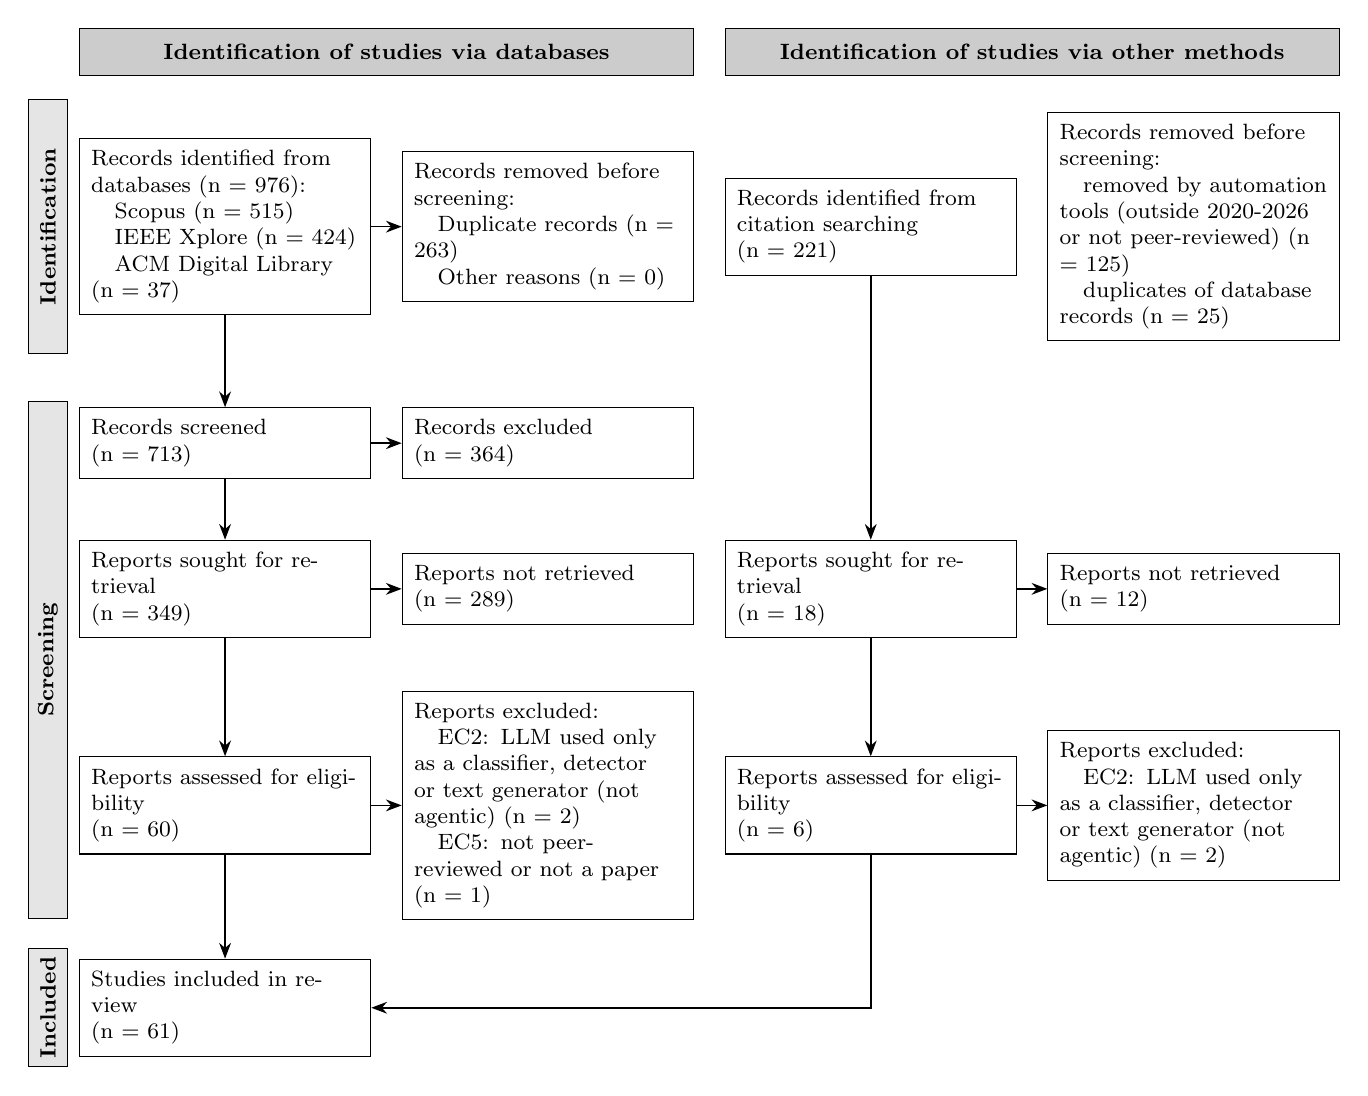
\begin{tikzpicture}[font=\footnotesize,
  box/.style={draw, fill=white, text width=3.4cm, align=left, inner sep=1.5mm},
  head/.style={draw, fill=black!20, minimum height=6mm, inner sep=1mm, font=\footnotesize\bfseries},
  phase/.style={draw, fill=black!10, minimum height=5mm, inner sep=1mm, rotate=90, font=\footnotesize\bfseries},
  arr/.style={-{Stealth[length=2mm]}, semithick}]
\node[head, minimum width=7.8cm] at (2.05,-0.3) {Identification of studies via databases};
\node[head, minimum width=7.8cm] at (10.25,-0.3) {Identification of studies via other methods};
\node[box] (ident) at (0.00,-2.52) {Records identified from databases (n = 976): \\ \hspace*{1em}Scopus (n = 515) \\ \hspace*{1em}IEEE Xplore (n = 424) \\ \hspace*{1em}ACM Digital Library (n = 37)};
\node[box] (removed) at (4.10,-2.52) {Records removed before screening: \\ \hspace*{1em}Duplicate records (n = 263) \\ \hspace*{1em}Other reasons (n = 0)};
\node[box] (cident) at (8.20,-2.52) {Records identified from citation searching \\ (n = 221)};
\node[box] (cremoved) at (12.30,-2.52) {Records removed before screening: \\ \hspace*{1em}removed by automation tools (outside 2020-2026 or not peer-reviewed) (n = 125) \\ \hspace*{1em}duplicates of database records (n = 25)};
\node[box] (screened) at (0.00,-5.27) {Records screened \\ (n = 713)};
\node[box] (exta) at (4.10,-5.27) {Records excluded \\ (n = 364)};
\node[box] (sought) at (0.00,-7.12) {Reports sought for retrieval \\ (n = 349)};
\node[box] (notret) at (4.10,-7.12) {Reports not retrieved \\ (n = 289)};
\node[box] (csought) at (8.20,-7.12) {Reports sought for retrieval \\ (n = 18)};
\node[box] (cnotret) at (12.30,-7.12) {Reports not retrieved \\ (n = 12)};
\node[box] (assessed) at (0.00,-9.87) {Reports assessed for eligibility \\ (n = 60)};
\node[box] (ftex) at (4.10,-9.87) {Reports excluded: \\ \hspace*{1em}EC2: LLM used only as a classifier, detector or text generator (not agentic) (n = 2) \\ \hspace*{1em}EC5: not peer-reviewed or not a paper (n = 1)};
\node[box] (cassessed) at (8.20,-9.87) {Reports assessed for eligibility \\ (n = 6)};
\node[box] (cftex) at (12.30,-9.87) {Reports excluded: \\ \hspace*{1em}EC2: LLM used only as a classifier, detector or text generator (not agentic) (n = 2)};
\node[box] (included) at (0.00,-12.44) {Studies included in review \\ (n = 61)};
\node[phase, minimum width=3.23cm] at (-2.25,-2.52) {Identification};
\node[phase, minimum width=6.57cm] at (-2.25,-8.02) {Screening};
\node[phase, minimum width=1.07cm] at (-2.25,-12.44) {Included};
\draw[arr] (ident) -- (screened);
\draw[arr] (screened) -- (sought);
\draw[arr] (sought) -- (assessed);
\draw[arr] (assessed) -- (included);
\draw[arr] (ident) -- (removed);
\draw[arr] (screened) -- (exta);
\draw[arr] (sought) -- (notret);
\draw[arr] (assessed) -- (ftex);
\draw[arr] (cident) -- (csought);
\draw[arr] (csought) -- (cassessed);
\draw[arr] (csought) -- (cnotret);
\draw[arr] (cassessed) -- (cftex);
\draw[arr] (cassessed.south) |- (included.east);
\end{tikzpicture}}

  \caption{PRISMA 2020 flow of records through identification, screening, eligibility assessment, and inclusion.}
  \Description{Flow diagram with separate database and citation-searching branches. A total of 784 records were screened, 367 reports were sought, 66 reports were assessed, and 60 studies were included.}
  \label{fig:prisma}
\end{figure}

\subsection{Quality Assessment and Extraction}

Four questions assessed clarity of aims and security tasks; reproducibility of agent, model, and tool descriptions; adequacy of evaluation; and discussion of limitations, threats, and risks. Scores were Yes~(1), Partial~(0.5), or No~(0), producing totals from zero to four. There was no quality-based exclusion threshold. For conceptual papers and surveys, evaluation adequacy concerned the rigour of the argument or review method.

Codex and agy initially scored the included reports independently, with disagreements adjudicated by Codex. Their initial assessment used length-limited extracted text. Factual extraction was also AI-prefilled from extracted text, with section pointers and explicit attribution. Fields cover study type, tasks, domain and orientation, architecture, models and adaptation, autonomy and oversight, evaluation, artifact availability, risks, limitations, and future work.

The author subsequently defined the categorical codebook. Architecture permits single-agent, multi-agent, mixed for studies evaluating both, and not applicable where no agent is implemented. Task stages and adaptation techniques are multi-label. Later verification compares complete papers and linked artifacts through two independent AI reviews and cross-review, preserving unresolved source inconsistencies.

At manuscript finalization, the two-AI workflow had reviewed all included extraction rows, QA scores and categorical codes, and all 420 final-code cells were populated. Individual author confirmation and the author-only gap and annotation fields remain incomplete. Consequently, category frequencies still describe a provisional AI-reviewed workbook snapshot. AI agreement is not treated as independent human validation, and no final corpus-wide comparative claim is inferred solely from those frequencies.


\section{Taxonomy}\label{sec:taxonomy}
% [YOU] Section 4 Taxonomy -- author-written; the taxonomy must be your own synthesis.
% Must contain: the organising framework; definitions of each dimension; a non-trivial taxonomy figure;
% the mapping of the included works to categories.

\begin{figure}[htbp]
  \centering
  % [YOU] Taxonomy figure (your own TikZ, or \includegraphics of your own drawing). Your original synthesis only.

  \caption{[YOU]}
  \Description{[YOU]}
  \label{fig:taxonomy}
\end{figure}


\section{Analysis by Category}\label{sec:analysis}
The synthesis below is deliberately bounded to studies whose complete reports and relevant artifacts have undergone the two-reviewer verification workflow. It therefore illustrates cross-study patterns without treating the still-provisional corpus frequencies as final evidence.

\subsection{Detection, Triage, Investigation, and Reporting}

Defensive agents increasingly combine specialized detectors with an LLM that coordinates retrieval and explanation. CyberRAG uses one central LLM agent to orchestrate attack-specific encoder classifiers, retrieval, reassessment, and report generation~\cite{R0447_Blefari_2026}. This architecture improved the reported unified payload-classification accuracy from 84.75\% for classifier-only selection to 94.92\% with LLaMA3.1:8B and RAG. The gain is not an end-to-end SOC result: explanation scoring begins from true attack labels, sample counts are missing, and the robustness denominator is inconsistent between text and figure caption.

OntoLogX addresses a different investigative unit: it converts logs into ontology-constrained knowledge graphs and predicts ATT\&CK tactics~\cite{R0365_Cotti_2026}. Retrieval and validation improve Claude Sonnet 4 KG F1 from 0.283 in the recorded baseline to 0.832 with a populated database, and the study releases code plus annotated data. Even this comparatively reproducible case retains contradictory reported values and an impossible printed construction-success ratio. \textbf{Critique:} accuracy or graph-quality improvements do not by themselves establish analyst benefit, streaming robustness, or resistance to adversarial telemetry. The verified evidence remains dominated by controlled payloads, curated logs, and offline scoring.

\subsection{Incident Response, Compliance, and Remediation}

The evidence separates three outcomes that are often conflated: generating advice, producing a corrected artifact, and applying a verified change. The RAN-compliance prototype generates and reflects on corrected configuration text, but live enforcement through the proposed SMO/O1 workflow is not evaluated~\cite{R0340_Chatzimiltis_2026}. Agentic RAG increases reported task accuracy across three models, while response time rises by approximately 74--189\%; the study also gives conflicting descriptions of how its ordinary-RAG queries are produced.

In autonomous network defense, architectural complexity is not uniformly beneficial. Across 3,475 CybORG CAGE-2 episodes, programmatic state abstraction improves one Llama configuration, whereas a distributed Devstral hierarchy worsens mean return and increases token use~\cite{R0484_Bogdanov_2026}. The result cautions against treating additional roles or deliberation as capability by default. \textbf{Critique:} the reviewed systems rarely connect a proposed action to transactional execution, rollback, and post-action validation. Corrected text and simulated rewards are useful intermediate evidence, but they should not be reported as demonstrated production remediation.

\subsection{Offensive and Penetration-Testing Workflows}

Offensive studies expose the strongest distinction between agent autonomy and LLM assistance. CurriculumPT implements a seven-agent workflow with tool execution, failure-aware replanning, curriculum scheduling, and retrieved experience~\cite{R0322_Wu_2025}. Its comparison table reports 60\% exploitation success, but a second table reports 66.7\% for another set also labelled as the 15-CVE hold-out evaluation. Its ablation percentages also cannot be reconstructed from ten once-tested CVEs per stratum without an unstated denominator or averaging procedure.

SatGuard, by contrast, is an empirical LLM-assisted penetration-testing workflow rather than an implemented software agent~\cite{R0384_Xiao_2025}. Testers submit scan output, copy generated commands into a CLI, and request follow-up analysis; consequently its architecture is coded not applicable under the review rule. The reported 22/30 successful attempts and 5.5 interactions per test measure a human-mediated process, and repair suggestions are not executed. \textbf{Critique:} task success must be accompanied by the intervention policy, supplied hints, retry rules, and action boundary. Otherwise a score can obscure whether the model completed a chain autonomously or helped a human complete it.

\subsection{Cross-Cutting Architecture and Evaluation Patterns}

The verified records show that ``single-agent'', ``multi-agent'', and ``mixed'' describe the evaluated control structure rather than the number of software modules. CyberRAG remains single-agent because its classifiers and retriever are tools; CurriculumPT is mixed at study level because it evaluates a focal multi-agent system against an agentic non-MAS comparator; and SatGuard has no implemented agent despite discussing conceptual autonomous variants. Prompting and retrieval commonly modify context rather than model weights, while fine-tuning may apply only to an auxiliary encoder.

Two reporting practices consistently improve interpretability: preserving the original evaluation unit and separating exact-study artifacts from dependencies. A public vulnerable VM or open framework does not establish release of prompts, run traces, splits, or interventions. Conversely, an exact repository may still be partial or inaccessible. \textbf{Critique:} cross-paper ranking is not defensible until denominators, stopping rules, human interventions, model versions, costs, and artifact scope are reported consistently.

\begin{table*}[tbp]
  \caption{Verified examples of task, architecture, and operational action boundaries.}\label{tab:comparison-1}
  \scriptsize
  \begin{tabular}{@{}p{0.14\textwidth}p{0.20\textwidth}p{0.15\textwidth}p{0.42\textwidth}@{}}
    \toprule
    Study & Primary task & Architecture & Verified operational boundary \\
    \midrule
    CyberRAG~\cite{R0447_Blefari_2026} & Alert triage, detection, reporting, advisory IR & Single-agent & Core LLM controls classifier and retrieval tools; mitigation and patch guidance are advisory; automated response is future work. \\
    OntoLogX~\cite{R0365_Cotti_2026} & CTI extraction and investigation & Single-agent & Generates, validates, and stores knowledge graphs; code, configuration, prompts, and annotations are released. \\
    RAN compliance~\cite{R0340_Chatzimiltis_2026} & Compliance reporting and artifact correction & Multi-agent & Produces corrected configuration text; live monitoring and enforcement remain proposed. \\
    Agent design study~\cite{R0484_Bogdanov_2026} & Simulated network defense & Mixed & Compares monolithic and hierarchical agents in CybORG; actions affect a simulated environment. \\
    CurriculumPT~\cite{R0322_Wu_2025} & Penetration testing and reporting & Mixed & Focal seven-agent system invokes tools and replans; human supplies the high-level objective; HITL maturity is internally inconsistent. \\
    SatGuard~\cite{R0384_Xiao_2025} & Penetration testing and reporting & Not applicable & Human submits scan output and executes generated commands; no autonomous controller or applied remediation is demonstrated. \\
    \bottomrule
  \end{tabular}
\end{table*}

\begin{table*}[tbp]
  \caption{Verified evaluation evidence and its principal qualification.}\label{tab:comparison-2}
  \scriptsize
  \begin{tabular}{@{}p{0.14\textwidth}p{0.27\textwidth}p{0.24\textwidth}p{0.26\textwidth}@{}}
    \toprule
    Study & Evaluation unit & Reported finding & Qualification / artifact scope \\
    \midrule
    CyberRAG~\cite{R0447_Blefari_2026} & Payload classification, conditional explanations, adversarial/OOD queries & 84.75\% to 94.92\% reported classification accuracy & Counts and one dataset identity are missing; SSTI archive is linked but password/access are unverified; framework code is not stated. \\
    OntoLogX~\cite{R0365_Cotti_2026} & 50 annotated AIT logs and 161 Cowrie sessions & Claude Sonnet 4 KG F1 reaches 0.832 in the populated-DB condition & Runnable code and annotations are public; several printed values conflict or are impossible. \\
    RAN compliance~\cite{R0340_Chatzimiltis_2026} & Four CU files, three repetitions, nine model/retrieval settings & Agentic-RAG accuracy exceeds No-RAG across three models & Only four files; annotation/scoring detail and uncertainty are incomplete; no live RAN test. \\
    Agent design study~\cite{R0484_Bogdanov_2026} & 3,475 CybORG episodes, 72 model/configuration pairs & Abstraction can improve return; hierarchy can worsen return and token cost & Configurations/prompts are released; original logs may be requested, while raw provider transcripts and seeds are not bundled. \\
    CurriculumPT~\cite{R0322_Wu_2025} & Curriculum, hold-out, and ablation CVE sets & Table 3 reports 60\% ESR versus 24--42\% baselines & Two N=15 hold-out tables conflict; ablation denominators are unreconciled; no exact-study release is stated. \\
    SatGuard~\cite{R0384_Xiao_2025} & 30 human-mediated exploitation attempts & 22/30 success; 5.5 interactions per test & No measured manual baseline, implemented agent, executed repair, or external study artifact. \\
    \bottomrule
  \end{tabular}
\end{table*}


\section{Datasets, Benchmarks and Evaluation}\label{sec:datasets}
\subsection{Evaluation Units and Environments}

The included evidence uses different evaluation units, including attack payloads, subtasks, vulnerable machines, CVE exploitation attempts, and simulated defender episodes. These units require separate interpretation. In the verified penetration-testing examples, Huang et al.\ evaluate tasks on HackTheBox, Metasploitable, and VulnHub machines, whereas CurriculumPT organizes Vulhub CVEs into a curriculum and separate evaluation sets~\cite{R0320_Huang_2025,R0322_Wu_2025}. The former lists 14 machines and 204 subtasks; the latter reports 50 curriculum CVEs, a 15-CVE hold-out set, and a 30-CVE ablation set. These counts do not establish equivalent task difficulty or independent trial counts.

Payload classification and explanation introduce another unit of analysis. CyberRAG combines SQL-injection and XSS resources with a constructed SSTI dataset, then evaluates classification, explanation quality, and robustness~\cite{R0447_Blefari_2026}. Its explanation evaluation begins with true attack labels, so those scores characterize conditional explanation quality rather than the complete classification-to-reporting pipeline.

Benchmark scope must also be distinguished from agent performance. The ATT\&CK coverage values examined by Missotten et al.\ describe the distribution of benchmark tasks across tactics, not the probability that an agent succeeds~\cite{R0249_Missotten_2025}. Simulated environments and public vulnerability platforms provide controlled conditions, but their results remain bounded by the available actions, task construction, and environment state.

\subsection{Metrics and Comparability}

The verified studies report exploitation or subtask success, accuracy, false positives, time, token use, human interventions, and explanation scores. Each measures a different aspect of the system. A success rate depends on its denominator, stopping rule, permitted tools, available hints, and treatment of partial progress. Time and token costs also depend on whether failed attempts are included and which model and orchestration settings are used.

Source inconsistencies are retained rather than silently reconciled. CurriculumPT reports different results for two tables labelled as a 15-CVE hold-out evaluation, while its ablation percentages require an aggregation explanation beyond the stated once-per-CVE design~\cite{R0322_Wu_2025}. Huang et al.\ likewise report modular-agent aggregate completion rates that are not reconciled with their task-category results~\cite{R0320_Huang_2025}. These results remain author-reported values with qualifications.

Operational outcomes need equally careful interpretation. Kulambayev et al.'s remediation-time values come from simulated workflows rather than observed production patch deployment~\cite{R0311_Kulambayev_2026}. PenHeal evaluates the value of recommended remediation strategies without executing those strategies~\cite{R0315_Huang_2024}. Neither result directly measures the safety or effectiveness of unattended remediation in an operational network.

Because tasks, denominators, environments, and outcomes differ, this review does not estimate a pooled effectiveness measure. Results are retained in their original units and interpreted alongside their baselines, implementation scope, and quality-assessment qualifications.

\subsection{Reproducibility and Artifact Scope}

Artifact availability is recorded separately for code and data. A public dependency, dataset homepage, or later follow-up repository is not automatically a release of the evaluated system. Similarly, ``not stated'' is distinguished from an explicit statement of unavailability, and on-request access is distinguished from an openly downloadable artifact.

The verified examples illustrate different levels of access. The compound-agent design study releases executable code and configurations, while original seeds and complete provider transcripts are not bundled~\cite{R0484_Bogdanov_2026}. CyberRAG links its constructed SSTI dataset, but the cited repository contains a password-described archive whose contents and access were not verified; this does not establish release of the complete framework or all evaluation sets~\cite{R0447_Blefari_2026}.

The extraction record therefore preserves exact model identifiers where available, tool and environment configuration, task manifests, prompts, stopping rules, raw-trace availability, and the relationship between an artifact and the study. Record-level two-AI review is complete, but corpus-wide availability percentages remain provisional until individual human confirmation.


\section{Open Problems and Research Agenda}\label{sec:open-problems}
% [YOU] Section 7 Open problems and research agenda -- author-written.
% Must contain: research gaps derived from empty taxonomy cells and from the critique in Section 5;
% concrete future directions; and it must cover ethics, fairness, reproducibility, and the safety and
% dual-use risks of autonomous response.


\section{Conclusion}\label{sec:conclusion}
% [YOU] Section 8 Conclusion -- author-written.
% Must contain: what the review establishes, and for whom. No new material.


\section{Threats to Validity}\label{sec:threats}
% [YOU] Threats to validity -- author-written.
% Must contain: an honest account of this review's own limitations (e.g. search, database, language and venue
% bias; single-screener bias) and the mitigations used.


% refs.bib is the Zotero Better BibTeX auto-export target. Never type an entry by hand or from memory.
\bibliographystyle{ACM-Reference-Format}
\bibliography{refs}

\appendix

\section{Search Strings}\label{app:search-strings}
% GENERATED from data/raw/search_strings_final_2026-10-29.md (verbatim strings, query v14). ACM row filled 2026-10-29.
All searches were run on 2026-10-29 with the publication years limited to 2020--2026. Strings are reproduced exactly as submitted; source-only line breaks were added at spaces for typesetting and do not change the queries.
\begin{table}[htbp]\centering\caption{Databases searched, filters and hits (query v14).}\label{tab:search-hits}
\begin{tabular}{lll}\toprule Source & Fields / filters & Hits \\ \midrule
Scopus & TITLE-ABS-KEY; ar, cp; English & 515 \\
IEEE Xplore & Title/Abstract/Index Terms; Conf., Journals, Early Access, Magazines & 424 (union of 3 queries) \\
ACM DL & Title/Abstract/Keyword; no type filter & 37 \\
Citation searching & OpenAlex, 5 seeds, backward + forward; peer-reviewed, 2020--2026 & 96 (221 retrieved) \\
\bottomrule\end{tabular}\end{table}
\subsection*{Scopus}
\begin{lstlisting}
TITLE-ABS-KEY ( ( ( "large language model*" OR llm OR llms OR "foundation model*" OR "generative AI"
OR "generative artificial intelligence" OR gpt* ) AND ( cybersecurity OR "cyber security" OR "cyber
defen*" OR "cyber-defen*" OR "network security" OR "security operation* cent*" OR siem OR soar OR
"cyber attack*" OR cyberattack* OR "network defen*" ) AND ( "intrusion detection" OR "anomaly
detection" OR "threat detection" OR "attack detection" OR "threat hunting" OR "alert triage" OR
"incident response" OR "incident handling" OR "attack investigation" OR remediation OR "security
orchestration" OR "autonomous response" OR "log analysis" OR "penetration test*" OR pentest* OR "red
team*" OR "attack emulation" OR "threat intelligence" OR cti OR forensic* OR "post-incident" OR
"cyber defen*" OR "network defen*" OR "active defen*" OR "defensive action*" OR "security
operation*" ) AND ( agentic OR "AI agent*" OR "LLM agent*" OR "LLM-based agent*" OR "autonomous
agent*" OR "multi-agent" OR multiagent OR "tool use" OR "tool-augmented" OR autonomous OR autonomy )
) OR ( ( "large language model*" OR llm OR llms OR "foundation model*" OR "generative AI" OR
"generative artificial intelligence" OR gpt* ) AND ( "penetration test*" OR pentest* ) ) ) AND
PUBYEAR > 2019 AND PUBYEAR < 2027 AND ( LIMIT-TO ( DOCTYPE , "ar" ) OR LIMIT-TO ( DOCTYPE , "cp" ) )
AND ( LIMIT-TO ( LANGUAGE , "English" ) )
\end{lstlisting}
\subsection*{IEEE Xplore}
\noindent\textit{A (= v13)}
\begin{lstlisting}
(("Document Title":"large language model*" OR "Abstract":"large language model*" OR "Index
Terms":"large language model*" OR "Document Title":llm OR "Abstract":llm OR "Index Terms":llm OR
"Document Title":llms OR "Abstract":llms OR "Index Terms":llms OR "Document Title":"foundation
model*" OR "Abstract":"foundation model*" OR "Index Terms":"foundation model*" OR "Document
Title":"generative AI" OR "Abstract":"generative AI" OR "Index Terms":"generative AI" OR "Document
Title":"generative artificial intelligence" OR "Abstract":"generative artificial intelligence" OR
"Index Terms":"generative artificial intelligence" OR "Document Title":gpt* OR "Abstract":gpt* OR
"Index Terms":gpt*) AND ("Document Title":cybersecurity OR "Abstract":cybersecurity OR "Index
Terms":cybersecurity OR "Document Title":"cyber security" OR "Abstract":"cyber security" OR "Index
Terms":"cyber security" OR "Document Title":"cyber defen*" OR "Abstract":"cyber defen*" OR "Index
Terms":"cyber defen*" OR "Document Title":"cyber-defen*" OR "Abstract":"cyber-defen*" OR "Index
Terms":"cyber-defen*" OR "Document Title":"network security" OR "Abstract":"network security" OR
"Index Terms":"network security" OR "Document Title":"security operation* cent*" OR
"Abstract":"security operation* cent*" OR "Index Terms":"security operation* cent*" OR "Document
Title":siem OR "Abstract":siem OR "Index Terms":siem OR "Document Title":soar OR "Abstract":soar OR
"Index Terms":soar OR "Document Title":"cyber attack*" OR "Abstract":"cyber attack*" OR "Index
Terms":"cyber attack*" OR "Document Title":cyberattack* OR "Abstract":cyberattack* OR "Index
Terms":cyberattack*) AND ("Document Title":"intrusion detection" OR "Abstract":"intrusion detection"
OR "Index Terms":"intrusion detection" OR "Document Title":"anomaly detection" OR
"Abstract":"anomaly detection" OR "Index Terms":"anomaly detection" OR "Document Title":"threat
detection" OR "Abstract":"threat detection" OR "Index Terms":"threat detection" OR "Document
Title":"attack detection" OR "Abstract":"attack detection" OR "Index Terms":"attack detection" OR
"Document Title":"threat hunting" OR "Abstract":"threat hunting" OR "Index Terms":"threat hunting"
OR "Document Title":"alert triage" OR "Abstract":"alert triage" OR "Index Terms":"alert triage" OR
"Document Title":"incident response" OR "Abstract":"incident response" OR "Index Terms":"incident
response" OR "Document Title":"incident handling" OR "Abstract":"incident handling" OR "Index
Terms":"incident handling" OR "Document Title":"attack investigation" OR "Abstract":"attack
investigation" OR "Index Terms":"attack investigation" OR "Document Title":remediation OR
"Abstract":remediation OR "Index Terms":remediation OR "Document Title":"security orchestration" OR
"Abstract":"security orchestration" OR "Index Terms":"security orchestration" OR "Document
Title":"autonomous response" OR "Abstract":"autonomous response" OR "Index Terms":"autonomous
response" OR "Document Title":"log analysis" OR "Abstract":"log analysis" OR "Index Terms":"log
analysis" OR "Document Title":"penetration test*" OR "Abstract":"penetration test*" OR "Index
Terms":"penetration test*" OR "Document Title":pentest* OR "Abstract":pentest* OR "Index
Terms":pentest* OR "Document Title":"red team*" OR "Abstract":"red team*" OR "Index Terms":"red
team*" OR "Document Title":"attack emulation" OR "Abstract":"attack emulation" OR "Index
Terms":"attack emulation" OR "Document Title":"threat intelligence" OR "Abstract":"threat
intelligence" OR "Index Terms":"threat intelligence" OR "Document Title":cti OR "Abstract":cti OR
"Index Terms":cti OR "Document Title":forensic* OR "Abstract":forensic* OR "Index Terms":forensic*
OR "Document Title":"post-incident" OR "Abstract":"post-incident" OR "Index Terms":"post-incident")
AND ("Document Title":agentic OR "Abstract":agentic OR "Index Terms":agentic OR "Document Title":"AI
agent*" OR "Abstract":"AI agent*" OR "Index Terms":"AI agent*" OR "Document Title":"LLM agent*" OR
"Abstract":"LLM agent*" OR "Index Terms":"LLM agent*" OR "Document Title":"LLM-based agent*" OR
"Abstract":"LLM-based agent*" OR "Index Terms":"LLM-based agent*" OR "Document Title":"autonomous
agent*" OR "Abstract":"autonomous agent*" OR "Index Terms":"autonomous agent*" OR "Document
Title":"multi-agent" OR "Abstract":"multi-agent" OR "Index Terms":"multi-agent" OR "Document
Title":multiagent OR "Abstract":multiagent OR "Index Terms":multiagent OR "Document Title":"tool
use" OR "Abstract":"tool use" OR "Index Terms":"tool use" OR "Document Title":"tool-augmented" OR
"Abstract":"tool-augmented" OR "Index Terms":"tool-augmented" OR "Document Title":autonomous OR
"Abstract":autonomous OR "Index Terms":autonomous OR "Document Title":autonomy OR
"Abstract":autonomy OR "Index Terms":autonomy)) OR (("Document Title":"large language model*" OR
"Abstract":"large language model*" OR "Index Terms":"large language model*" OR "Document Title":llm
OR "Abstract":llm OR "Index Terms":llm OR "Document Title":llms OR "Abstract":llms OR "Index
Terms":llms OR "Document Title":"foundation model*" OR "Abstract":"foundation model*" OR "Index
Terms":"foundation model*" OR "Document Title":"generative AI" OR "Abstract":"generative AI" OR
"Index Terms":"generative AI" OR "Document Title":"generative artificial intelligence" OR
"Abstract":"generative artificial intelligence" OR "Index Terms":"generative artificial
intelligence" OR "Document Title":gpt* OR "Abstract":gpt* OR "Index Terms":gpt*) AND ("Document
Title":"penetration test*" OR "Abstract":"penetration test*" OR "Index Terms":"penetration test*" OR
"Document Title":pentest* OR "Abstract":pentest* OR "Index Terms":pentest*))
\end{lstlisting}
\noindent\textit{B1}
\begin{lstlisting}
("Document Title":"large language model*" OR "Abstract":"large language model*" OR "Index
Terms":"large language model*" OR "Document Title":llm OR "Abstract":llm OR "Index Terms":llm OR
"Document Title":llms OR "Abstract":llms OR "Index Terms":llms OR "Document Title":"foundation
model*" OR "Abstract":"foundation model*" OR "Index Terms":"foundation model*" OR "Document
Title":"generative AI" OR "Abstract":"generative AI" OR "Index Terms":"generative AI" OR "Document
Title":"generative artificial intelligence" OR "Abstract":"generative artificial intelligence" OR
"Index Terms":"generative artificial intelligence" OR "Document Title":gpt* OR "Abstract":gpt* OR
"Index Terms":gpt*) AND ("Document Title":agentic OR "Abstract":agentic OR "Index Terms":agentic OR
"Document Title":"AI agent*" OR "Abstract":"AI agent*" OR "Index Terms":"AI agent*" OR "Document
Title":"LLM agent*" OR "Abstract":"LLM agent*" OR "Index Terms":"LLM agent*" OR "Document
Title":"LLM-based agent*" OR "Abstract":"LLM-based agent*" OR "Index Terms":"LLM-based agent*" OR
"Document Title":"autonomous agent*" OR "Abstract":"autonomous agent*" OR "Index Terms":"autonomous
agent*" OR "Document Title":"multi-agent" OR "Abstract":"multi-agent" OR "Index Terms":"multi-agent"
OR "Document Title":multiagent OR "Abstract":multiagent OR "Index Terms":multiagent OR "Document
Title":"tool use" OR "Abstract":"tool use" OR "Index Terms":"tool use" OR "Document
Title":"tool-augmented" OR "Abstract":"tool-augmented" OR "Index Terms":"tool-augmented" OR
"Document Title":autonomous OR "Abstract":autonomous OR "Index Terms":autonomous OR "Document
Title":autonomy OR "Abstract":autonomy OR "Index Terms":autonomy) AND ("Document
Title":cybersecurity OR "Abstract":cybersecurity OR "Index Terms":cybersecurity OR "Document
Title":"cyber security" OR "Abstract":"cyber security" OR "Index Terms":"cyber security" OR
"Document Title":"cyber defen*" OR "Abstract":"cyber defen*" OR "Index Terms":"cyber defen*" OR
"Document Title":"cyber-defen*" OR "Abstract":"cyber-defen*" OR "Index Terms":"cyber-defen*" OR
"Document Title":"network security" OR "Abstract":"network security" OR "Index Terms":"network
security" OR "Document Title":"security operation* cent*" OR "Abstract":"security operation* cent*"
OR "Index Terms":"security operation* cent*" OR "Document Title":siem OR "Abstract":siem OR "Index
Terms":siem OR "Document Title":soar OR "Abstract":soar OR "Index Terms":soar OR "Document
Title":"cyber attack*" OR "Abstract":"cyber attack*" OR "Index Terms":"cyber attack*" OR "Document
Title":cyberattack* OR "Abstract":cyberattack* OR "Index Terms":cyberattack* OR "Document
Title":"network defen*" OR "Abstract":"network defen*" OR "Index Terms":"network defen*") AND
("Document Title":"cyber defen*" OR "Abstract":"cyber defen*" OR "Index Terms":"cyber defen*" OR
"Document Title":"network defen*" OR "Abstract":"network defen*" OR "Index Terms":"network defen*"
OR "Document Title":"active defen*" OR "Abstract":"active defen*" OR "Index Terms":"active defen*"
OR "Document Title":"defensive action*" OR "Abstract":"defensive action*" OR "Index
Terms":"defensive action*" OR "Document Title":"security operation*" OR "Abstract":"security
operation*" OR "Index Terms":"security operation*")
\end{lstlisting}
\noindent\textit{B2}
\begin{lstlisting}
("Document Title":"large language model*" OR "Abstract":"large language model*" OR "Index
Terms":"large language model*" OR "Document Title":llm OR "Abstract":llm OR "Index Terms":llm OR
"Document Title":llms OR "Abstract":llms OR "Index Terms":llms OR "Document Title":"foundation
model*" OR "Abstract":"foundation model*" OR "Index Terms":"foundation model*" OR "Document
Title":"generative AI" OR "Abstract":"generative AI" OR "Index Terms":"generative AI" OR "Document
Title":"generative artificial intelligence" OR "Abstract":"generative artificial intelligence" OR
"Index Terms":"generative artificial intelligence" OR "Document Title":gpt* OR "Abstract":gpt* OR
"Index Terms":gpt*) AND ("Document Title":agentic OR "Abstract":agentic OR "Index Terms":agentic OR
"Document Title":"AI agent*" OR "Abstract":"AI agent*" OR "Index Terms":"AI agent*" OR "Document
Title":"LLM agent*" OR "Abstract":"LLM agent*" OR "Index Terms":"LLM agent*" OR "Document
Title":"LLM-based agent*" OR "Abstract":"LLM-based agent*" OR "Index Terms":"LLM-based agent*" OR
"Document Title":"autonomous agent*" OR "Abstract":"autonomous agent*" OR "Index Terms":"autonomous
agent*" OR "Document Title":"multi-agent" OR "Abstract":"multi-agent" OR "Index Terms":"multi-agent"
OR "Document Title":multiagent OR "Abstract":multiagent OR "Index Terms":multiagent OR "Document
Title":"tool use" OR "Abstract":"tool use" OR "Index Terms":"tool use" OR "Document
Title":"tool-augmented" OR "Abstract":"tool-augmented" OR "Index Terms":"tool-augmented" OR
"Document Title":autonomous OR "Abstract":autonomous OR "Index Terms":autonomous OR "Document
Title":autonomy OR "Abstract":autonomy OR "Index Terms":autonomy) AND ("Document Title":"network
defen*" OR "Abstract":"network defen*" OR "Index Terms":"network defen*") AND ("Document
Title":"intrusion detection" OR "Abstract":"intrusion detection" OR "Index Terms":"intrusion
detection" OR "Document Title":"anomaly detection" OR "Abstract":"anomaly detection" OR "Index
Terms":"anomaly detection" OR "Document Title":"threat detection" OR "Abstract":"threat detection"
OR "Index Terms":"threat detection" OR "Document Title":"attack detection" OR "Abstract":"attack
detection" OR "Index Terms":"attack detection" OR "Document Title":"threat hunting" OR
"Abstract":"threat hunting" OR "Index Terms":"threat hunting" OR "Document Title":"alert triage" OR
"Abstract":"alert triage" OR "Index Terms":"alert triage" OR "Document Title":"incident response" OR
"Abstract":"incident response" OR "Index Terms":"incident response" OR "Document Title":"incident
handling" OR "Abstract":"incident handling" OR "Index Terms":"incident handling" OR "Document
Title":"attack investigation" OR "Abstract":"attack investigation" OR "Index Terms":"attack
investigation" OR "Document Title":remediation OR "Abstract":remediation OR "Index
Terms":remediation OR "Document Title":"security orchestration" OR "Abstract":"security
orchestration" OR "Index Terms":"security orchestration" OR "Document Title":"autonomous response"
OR "Abstract":"autonomous response" OR "Index Terms":"autonomous response" OR "Document Title":"log
analysis" OR "Abstract":"log analysis" OR "Index Terms":"log analysis" OR "Document
Title":"penetration test*" OR "Abstract":"penetration test*" OR "Index Terms":"penetration test*" OR
"Document Title":pentest* OR "Abstract":pentest* OR "Index Terms":pentest* OR "Document Title":"red
team*" OR "Abstract":"red team*" OR "Index Terms":"red team*" OR "Document Title":"attack emulation"
OR "Abstract":"attack emulation" OR "Index Terms":"attack emulation" OR "Document Title":"threat
intelligence" OR "Abstract":"threat intelligence" OR "Index Terms":"threat intelligence" OR
"Document Title":cti OR "Abstract":cti OR "Index Terms":cti OR "Document Title":forensic* OR
"Abstract":forensic* OR "Index Terms":forensic* OR "Document Title":"post-incident" OR
"Abstract":"post-incident" OR "Index Terms":"post-incident")
\end{lstlisting}
\subsection*{ACM Digital Library}
\begin{lstlisting}
((Title:("large language model" OR "large language models" OR llm OR llms OR "foundation model" OR
"foundation models" OR "generative AI" OR "generative artificial intelligence" OR gpt*) OR
Abstract:("large language model" OR "large language models" OR llm OR llms OR "foundation model" OR
"foundation models" OR "generative AI" OR "generative artificial intelligence" OR gpt*) OR
Keyword:("large language model" OR "large language models" OR llm OR llms OR "foundation model" OR
"foundation models" OR "generative AI" OR "generative artificial intelligence" OR gpt*)) AND
(Title:(cybersecurity OR "cyber security" OR "cyber defense" OR "cyber defence" OR "cyber-defense"
OR "cyber-defence" OR "network security" OR "security operations center" OR "security operation
center" OR "security operations centre" OR siem OR soar OR "cyber attack" OR "cyber attacks" OR
cyberattack* OR "network defense" OR "network defence") OR Abstract:(cybersecurity OR "cyber
security" OR "cyber defense" OR "cyber defence" OR "cyber-defense" OR "cyber-defence" OR "network
security" OR "security operations center" OR "security operation center" OR "security operations
centre" OR siem OR soar OR "cyber attack" OR "cyber attacks" OR cyberattack* OR "network defense" OR
"network defence") OR Keyword:(cybersecurity OR "cyber security" OR "cyber defense" OR "cyber
defence" OR "cyber-defense" OR "cyber-defence" OR "network security" OR "security operations center"
OR "security operation center" OR "security operations centre" OR siem OR soar OR "cyber attack" OR
"cyber attacks" OR cyberattack* OR "network defense" OR "network defence")) AND (Title:("intrusion
detection" OR "anomaly detection" OR "threat detection" OR "attack detection" OR "threat hunting" OR
"alert triage" OR "incident response" OR "incident handling" OR "attack investigation" OR
remediation OR "security orchestration" OR "autonomous response" OR "log analysis" OR "penetration
test" OR "penetration testing" OR "penetration tests" OR pentest* OR "red team" OR "red teaming" OR
"red teams" OR "attack emulation" OR "threat intelligence" OR cti OR forensic* OR "post-incident" OR
"cyber defense" OR "cyber defence" OR "network defense" OR "network defence" OR "active defense" OR
"active defence" OR "defensive action" OR "defensive actions" OR "security operation" OR "security
operations") OR Abstract:("intrusion detection" OR "anomaly detection" OR "threat detection" OR
"attack detection" OR "threat hunting" OR "alert triage" OR "incident response" OR "incident
handling" OR "attack investigation" OR remediation OR "security orchestration" OR "autonomous
response" OR "log analysis" OR "penetration test" OR "penetration testing" OR "penetration tests" OR
pentest* OR "red team" OR "red teaming" OR "red teams" OR "attack emulation" OR "threat
intelligence" OR cti OR forensic* OR "post-incident" OR "cyber defense" OR "cyber defence" OR
"network defense" OR "network defence" OR "active defense" OR "active defence" OR "defensive action"
OR "defensive actions" OR "security operation" OR "security operations") OR Keyword:("intrusion
detection" OR "anomaly detection" OR "threat detection" OR "attack detection" OR "threat hunting" OR
"alert triage" OR "incident response" OR "incident handling" OR "attack investigation" OR
remediation OR "security orchestration" OR "autonomous response" OR "log analysis" OR "penetration
test" OR "penetration testing" OR "penetration tests" OR pentest* OR "red team" OR "red teaming" OR
"red teams" OR "attack emulation" OR "threat intelligence" OR cti OR forensic* OR "post-incident" OR
"cyber defense" OR "cyber defence" OR "network defense" OR "network defence" OR "active defense" OR
"active defence" OR "defensive action" OR "defensive actions" OR "security operation" OR "security
operations")) AND (Title:(agentic OR "AI agent" OR "AI agents" OR "LLM agent" OR "LLM agents" OR
"LLM-based agent" OR "LLM-based agents" OR "autonomous agent" OR "autonomous agents" OR
"multi-agent" OR multiagent OR "tool use" OR "tool-augmented" OR autonomous OR autonomy) OR
Abstract:(agentic OR "AI agent" OR "AI agents" OR "LLM agent" OR "LLM agents" OR "LLM-based agent"
OR "LLM-based agents" OR "autonomous agent" OR "autonomous agents" OR "multi-agent" OR multiagent OR
"tool use" OR "tool-augmented" OR autonomous OR autonomy) OR Keyword:(agentic OR "AI agent" OR "AI
agents" OR "LLM agent" OR "LLM agents" OR "LLM-based agent" OR "LLM-based agents" OR "autonomous
agent" OR "autonomous agents" OR "multi-agent" OR multiagent OR "tool use" OR "tool-augmented" OR
autonomous OR autonomy))) OR ((Title:("large language model" OR "large language models" OR llm OR
llms OR "foundation model" OR "foundation models" OR "generative AI" OR "generative artificial
intelligence" OR gpt*) OR Abstract:("large language model" OR "large language models" OR llm OR llms
OR "foundation model" OR "foundation models" OR "generative AI" OR "generative artificial
intelligence" OR gpt*) OR Keyword:("large language model" OR "large language models" OR llm OR llms
OR "foundation model" OR "foundation models" OR "generative AI" OR "generative artificial
intelligence" OR gpt*)) AND (Title:("penetration test" OR "penetration testing" OR "penetration
tests" OR pentest*) OR Abstract:("penetration test" OR "penetration testing" OR "penetration tests"
OR pentest*) OR Keyword:("penetration test" OR "penetration testing" OR "penetration tests" OR
pentest*)))
\end{lstlisting}


\section{PRISMA 2020 Checklist}\label{app:prisma-checklist}
\small
\begin{longtable}{@{}p{0.06\linewidth}p{0.27\linewidth}p{0.47\linewidth}p{0.14\linewidth}@{}}
\caption{PRISMA 2020 checklist mapping.}\label{tab:prisma-checklist}\\
\toprule
Item & Topic & Location in this review & Status \\
\midrule
\endfirsthead
\toprule
Item & Topic & Location in this review & Status \\
\midrule
\endhead
1 & Title & Manuscript title & Reported \\
2 & Abstract & Abstract & Reported \\
3 & Rationale & Section~\ref{sec:introduction} & Reported \\
4 & Objectives & Section~\ref{sec:introduction}, research questions & Reported \\
5 & Eligibility criteria & Section~\ref{sec:methodology}, Protocol and Scope & Reported \\
6 & Information sources & Section~\ref{sec:methodology}, Search and Record Processing & Reported \\
7 & Search strategy & Appendix~\ref{app:search-strings} & Reported verbatim \\
8 & Selection process & Section~\ref{sec:methodology}, Screening and Retrieval & Reported \\
9 & Data-collection process & Section~\ref{sec:methodology}, Quality Assessment and Extraction & Reported \\
10a & Outcomes sought & Section~\ref{sec:methodology}; extraction matrix & Reported \\
10b & Other variables & Section~\ref{sec:methodology}; codebook and extraction matrix & Reported \\
11 & Risk-of-bias assessment & Four-item QA instrument; Appendix QA table & Partial proxy \\
12 & Effect measures & Section~\ref{sec:datasets}; original study units retained & Not pooled \\
13a--f & Synthesis methods & Sections~\ref{sec:taxonomy}--\ref{sec:datasets}; no meta-analysis & Narrative \\
14 & Reporting-bias assessment & Threats to validity; artifact/reporting limitations & Qualitative \\
15 & Certainty assessment & No formal GRADE-style certainty assessment & Not performed \\
16a & Study selection & Figure~\ref{fig:prisma} & Reported \\
16b & Excluded reports & Full-text QA sheet and PRISMA counts (five EC2; one EC5) & Reported \\
17 & Study characteristics & Extraction matrix and comparison tables & Partial verification \\
18 & Risk of bias in studies & Appendix QA table & Reported \\
19 & Results of individual studies & Sections~\ref{sec:analysis}--\ref{sec:datasets}; extraction matrix & Verified subset \\
20a--d & Results of syntheses & Sections~\ref{sec:taxonomy}--\ref{sec:datasets} & Provisional \\
21 & Reporting biases & Threats to validity and reproducibility discussion & Qualitative \\
22 & Certainty of evidence & Not formally assessed & Not performed \\
23a & Interpretation & Sections~\ref{sec:analysis}--\ref{sec:conclusion} & Reported \\
23b & Limitations of evidence & Section~\ref{sec:datasets} and Threats to Validity & Reported \\
23c & Limitations of review & Threats to Validity & Reported \\
23d & Implications & Section~\ref{sec:open-problems} & Reported \\
24a & Registration & No prospective registration & Not registered \\
24b & Protocol access & Project repository; protocol and dated decision records & Reported \\
24c & Amendments & Methodology and protocol amendment log & Reported \\
25 & Support & No support declaration appears in the current manuscript & Not reported \\
26 & Competing interests & No competing-interest declaration appears in the current manuscript & Not reported \\
27 & Availability of materials & Data Availability statement & Reported \\
\bottomrule
\end{longtable}
\normalsize


\section{Quality-Assessment Scores}\label{app:qa-scores}
% [YOU] Appendix: quality-assessment scores.
% Must contain: the score of every included study on each quality criterion, and the total.


\section{Data Availability}\label{app:data-availability}
% [YOU] Data availability statement.
% Must contain: where the shared BibTeX, the extraction spreadsheet, the screening corpus and dedup log,
% the raw search exports and the scripts can be obtained.


\section{Use of AI Tools}\label{app:ai-use}
% [YOU] Use of AI tools (disclosure).
% Must contain: every AI tool used, the task it helped with, and whether its output was verified
% (mirror the "Use of AI Tools" table in the workbook).


\end{document}
